% ************ Chapter 4 ************
\chapter{Projeção do Sistema de Informação} 
\label{cap:4}
Levantados os requisitos do projeto, iniciou-se projeção do sistema. Este foi um processo que envolveu desde planeamento de trabalho a ser realizado, ao design da aplicação.

\section{Planeamento do projeto}
A primeira semana do período do estágio foram destinadas ao levantamento de requisitos. Foi ainda durante esta semana que ocorreu o redesign da base de dados.
As semanas 2 e 3 foram destinadas ao estudo dos \textit{frameworks} a utilizar, do sistema de gestão de base de dados e do ambiente da empresa.
Conforme indicado nos requisitos do projeto, o desenvolvimento do sistema de informação teria de ser dividido em duas fases. A data para a conclusão da primeira fase foi fixada no inicio da sexta semana, dando-se logo incio à fase dois.

\section{Design da nova base de dados}
A base de dados a ser utilizada neste projeto teve como ponto de partida aquela que já era utilizada pela aplicação antiga. De modo a tornar a estrutura o mais adequada possível, numa da reuniões, foi solicitado à administração que descrevesse em detalhe o fluxo de informação da estrutura até à data implementada. Após a reunião seguiu-se um estudo para encontrar formas de otimizar a estrutura da base de dados, não apenas na questão da normalização da estrutura mas também de forma a tornar o trabalho futuro mais simples procurando meios de otimizar o fluxo da informação. Após o estudo foi entregue de uma proposta da nova estrutura. Esta foi chumbada numa fase inicial porque, como resultado da normalização, foi criada uma tabela destinada a armazenar os cemitérios com os quais a empresa tem parceria, uma segunda tabela onde ficaram registadas as empresas a quem a Natural Life compra o materia-prima e uma terceira tabela responsável por agregar os registos das primeiras duas de modo a estabelecer as relações com a restantes tabelas do sistema. A reposta da administração foi que preferia que existisse apenas uma única tabela, que agregasse os campos das três referidas anteriormente, com um campo extra para distinguir o tipo de registo. Apesar de compreenderem qual era o intuito da mudança sugerida, esta iria tornar mais difícil a adaptação de ficheiros Excel e PowerBi já existentes. A mudança pedida foi efetuada e a administração aceitou as restantes alterações sugeridas. Dentre dela destaca-se a tabela "Entidades" criada para armazenar as informações de identificação (nome, morada, código postal e nif) dos pontos de recolha e clientes. Esta alteração permitiu não só reunir num único local a lista de entidades com as quais a Natural Life interage, eliminado eventuais incoerências de informação a respeito do numero de identificação fiscal, por exemplo.
O processo de reforma da base de dados manteve-se então congelado até à sétima semana, na qual se criou a tabela "completar\_recolha", conforme descrito no capítulo anterior. No final de todo este processo a estrutura final da base de dados, aprovada pela administração, é a descrita na figura \ref{fig:db_model}.

\begin{figure}[htbp] 
	\begin{center}
		% Requires \usepackage{graphicx}
		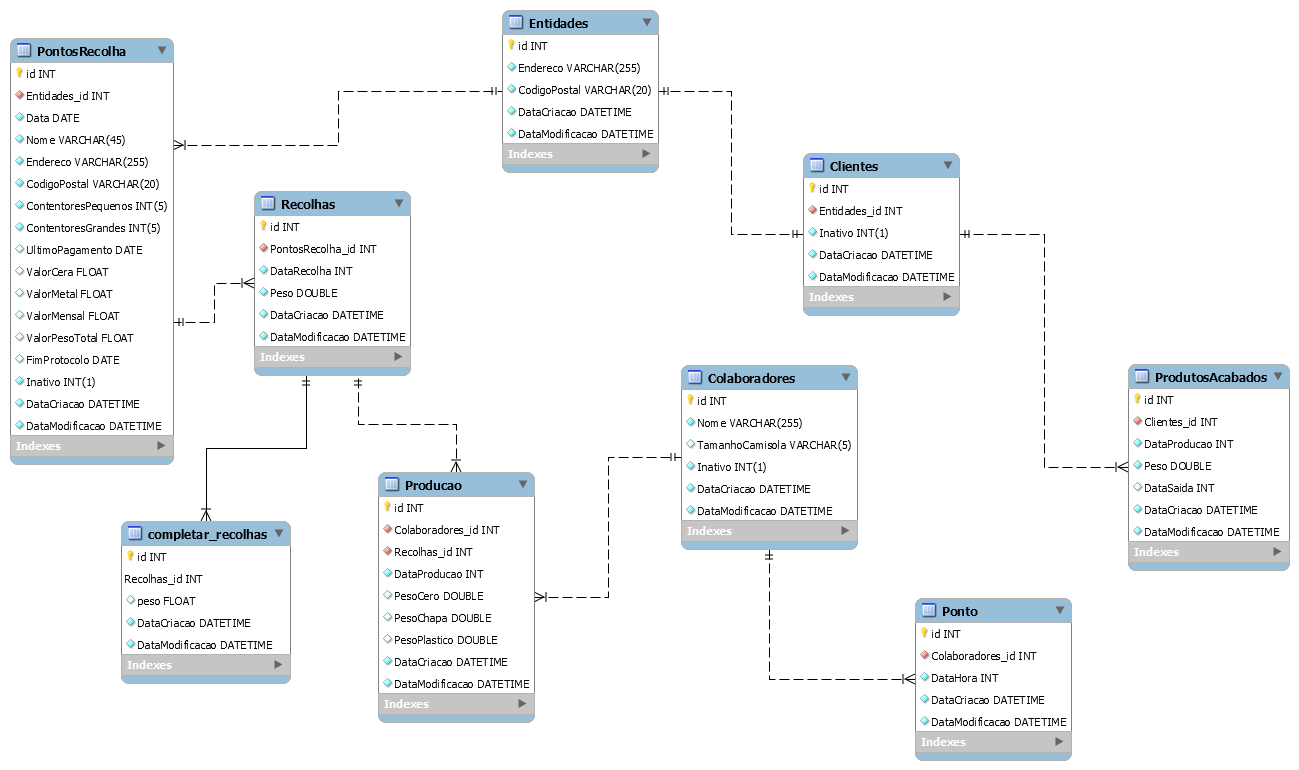
\includegraphics[width=\textwidth,keepaspectratio]{figuras/DB_Model/new.png}
		\caption{Estrutura final da base de dados}
		\label{fig:db_model} 
	\end{center}
\end{figure}

Finalizado este processo, iniciou-se o processo de design da aplicação.

\section{Aplicação}
Respondendo aos requisitos definidos no Capitulo \ref{cap:3}, a aplicação a ser desenvolvida seria uma aplicação web construída em PHP, com o framwork laravel, e JavaScript segundo o padrão do modelo MVC. O modelo MVC, representado na figura \ref{fig:mvc}, descreve a forma como uma aplicação deve ser construída separando-a em três camadas distintas: Model View e Controller. Esta separação server distinguir representações de informação internas dos modos como a informação é apresentada ao utilizador\cite{Wikipediad}.
Esta abstração em camadas é particularmente vantajosa no que toca a fazer reutilização de código, pois tendo em conta as regras do modelo cada classe tem apenas uma responsabilidade atribuída além de o projeto ter um baixo acoplamento entre si. Desta forma é muito fácil utilizar a mesma classe partes distas do projeto, facilitando a sua compreensão, manutenção e atualização.
Estas características do modelo servem ainda de resposta a outros requisitos do projeto como modularidade do projeto.
\begin{figure}[H] 
	\begin{center}
		% Requires \usepackage{graphicx}
		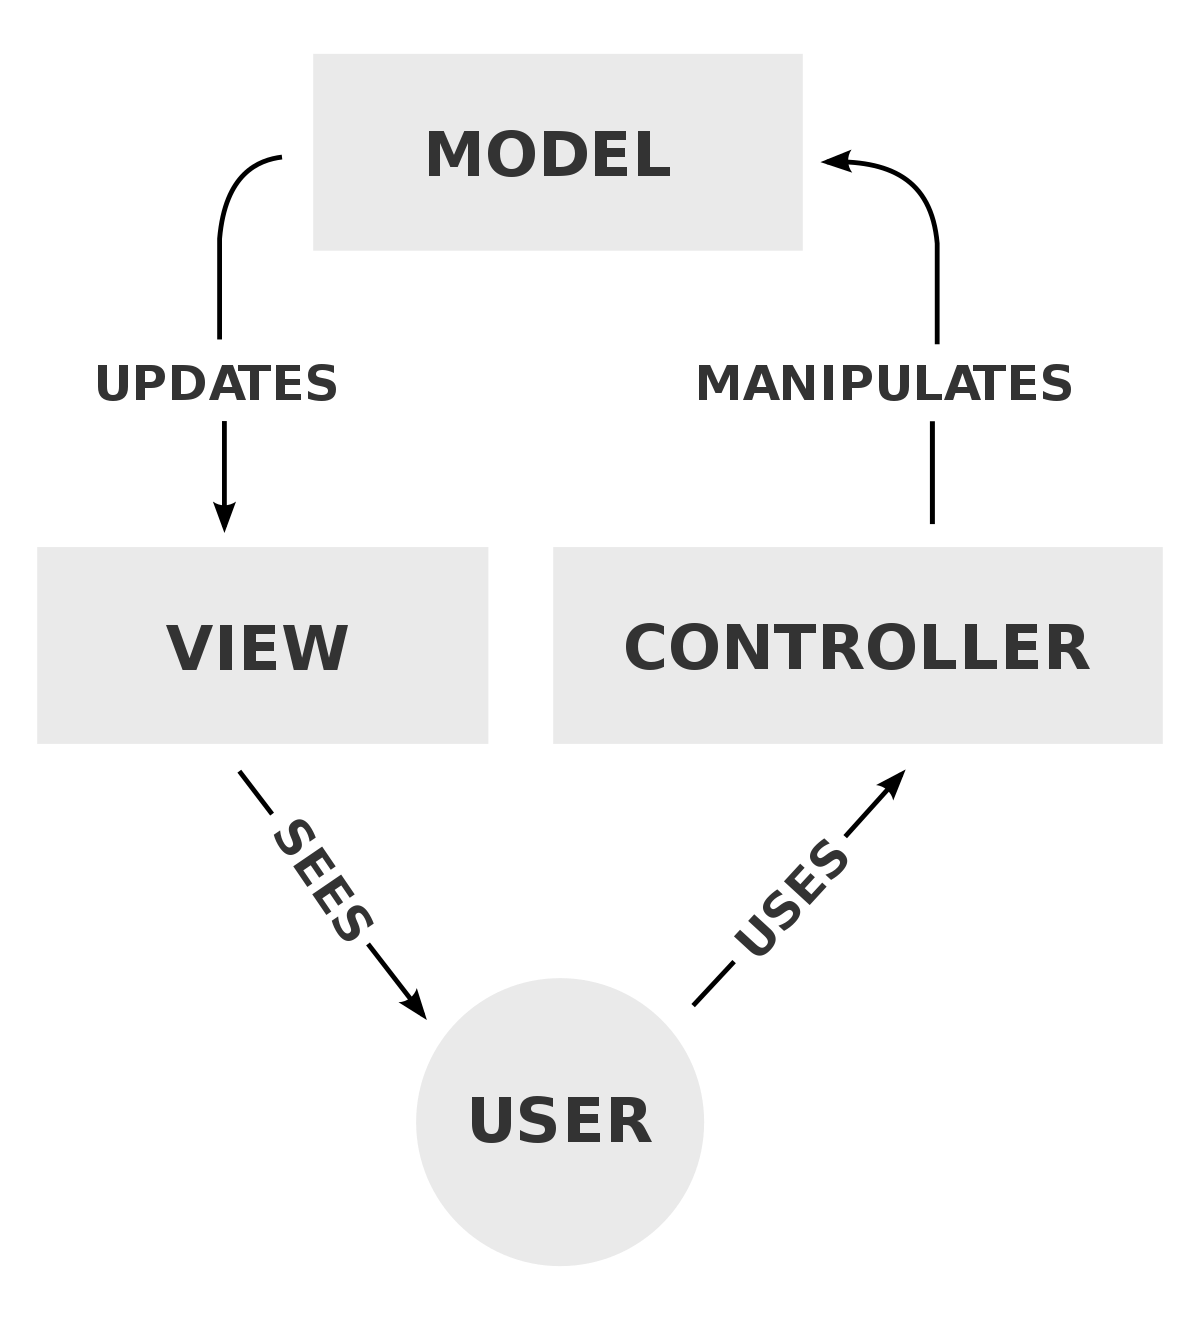
\includegraphics[width=0.30\textwidth,keepaspectratio]{figuras/mvc.png}
		\caption{Diagrama do modelo MVC}
		\label{fig:mvc} 
	\end{center}
\end{figure}

\noindent 
Ainda respondendo aos requisitos deveria existir duas áreas distintas dentro da aplicação destinada aos colaboradores na fábrica e à administração.
Estas suas sub-aplicações foram designadas de Aplicação Fábrica, acessível aos colaboradores da empresa e responsável pelos registos de informação na base de dados, e a Aplicação Painel, protegida por um sistema de autenticação na qual seria possível manipular toda a informação registada.
Para fazer esta separação, os endereços dentro da aplicação foram divididos em dois grupos distintos. Em primeiro lugar as páginas associadas à Aplicação de Fábrica estavam sob o endereço /Fabrica:

\begin{center}
\url{http://<ip.do.servidor>/Fabrica/<Nome_da_página_solicitada>}
\end{center}

\noindent 
Enquanto as páginas relacionadas com a Aplicação Painel estavam sob o endereço /Painel:

\begin{center}
	\url{http://<ip.do.servidor>/Painel/<Nome_da_página_solicitada>}
\end{center}

\noindent 
A única exceção a esta regra está no diretório raiz do sistema, que direciona para a página index da Aplicação de Fábrica.\\
Esta organização em nada muda a estrutura de ficheiros do projeto. O framework laravel, trás consigo um recurso de rotas, que permite facilmente que este tipo de regras seja incluída no projeto sem ter necessariamente que fazer modificações à árvore de diretórios da aplicação. Desta forma, manteve-se uma estrutura dos ficheiros da aplicação coesa, mantendo cada tipo de ficheiro na sua pasta definida e manter regras de padronização dos endereços da aplicação.

\section{Funcionalidades do sistema}
Definidos todos os detalhes supracitados, é possível dar inicio à definição de cada uma das funcionalidades do projeto. Esta definição serve como guia de desenvolvimento, mantendo as informações necessárias para se conhecer o comportamento esperado de cada uma das funcionalidades do sistema final.